% 请确保文件编码为utf-8,使用XeLaTex进行编译,或者通过overleaf进行编译

\documentclass[answers]{exam}  % 使用此行带有作答模块
% \documentclass{exam} % 使用此行只显示题目

\usepackage{xeCJK}
\usepackage{zhnumber}
\usepackage{graphicx}
\usepackage{hyperref}
\usepackage{amsmath}
\usepackage{amssymb}
\usepackage{mathtools}
\usepackage{booktabs}
\usepackage{enumerate}
\usepackage{enumitem} % 控制列表样式
\usepackage{listings} 
\usepackage{float}

\title{2025自然语言处理 \\ 课程设计1}
\date{2025.4.1}
\pagestyle{headandfoot}
\author{人工智能学院 221300079 王俊童}
\firstpageheadrule
\firstpageheader{南京大学}{2025自然语言处理}{课程设计1}
\runningheader{南京大学}
{2025自然语言处理}
{课程设计1}
\runningheadrule
\firstpagefooter{}{第\thepage\ 页(共\numpages 页)}{}
\runningfooter{}{第\thepage\ 页(共\numpages 页)}{}

% no box for solutions
% \unframedsolutions
\def \x \mathbf{x}


\setlength\linefillheight{.5in}

% \renewcommand{\solutiontitle}{\noindent\textbf{答:}}
\renewcommand{\solutiontitle}{\noindent\textbf{解:}\par\noindent}

\renewcommand{\thequestion}{\zhnum{question}}
\renewcommand{\questionlabel}{\thequestion .}
\renewcommand{\thepartno}{\arabic{partno}}
\renewcommand{\partlabel}{\thepartno .}

% 实验报告需包含以下内容:

% 实现了哪些方法并对自己设计的代码模块用简洁的语言描述
% 如何复现主要实现结果,包括执行命令和环境依赖,
% 建议修改requirement.txt和新建bash文件来展示如何运行代码
% 不同方法的实验结果如何
% 遇到的具体问题,如何解决
% 对该任务和在探索过程中的思考


\begin{document}
% \normalsize
\maketitle
\textbf{写在开头,请助教老师一定要看完这份报告。先说结果,方便老师评价,\\
    正常方法 F0.5: 0.1991 ± 0.0049,\\
    用了预训练模型(作弊方法) F0.5: 0.4120}

综述,首先观察代码结构,逻辑如下:
\begin{itemize}
    \item 命令行参数解析。有method,是否analyze,statistical里面方法的选取。
    \item 加载数据和数据分析(需要我们实现数据分析)
    \item 三个方法的训练:
    \begin{itemize}
        \item rule:基于一些规则得到的一个实现。train有四种纠错规则:
        \begin{itemize}
            \item $\_extract\_confusion\_pairs$:字符混淆对提取。
            \item $\_extract\_punctuation\_rules$:标点符号规则提取
            \item $\_extract\_grammar\_rules$:语法规则提取
            \item $\_extract\_word\_confusion$:词汇混淆对提取
        \end{itemize}
        然后以上四种错误的纠错发生在correct里面。
        \item statistical:基于统计学习方法的纠错。这个里面又分为两个模型:
        \begin{itemize}
            \item ngram模型:初始化了一堆数据结构,1-4的gram方法,字符混淆矩阵和错误率等
            \item ml模型:用机器学习方法去做。
        \end{itemize}
        \item 集成学习方法,在框架代码的ensemble部分有留给我们实现。
    \end{itemize}
    \item 三个方法对应的纠错和评估。跟上面一样了,可以实现很多的correct方法,都有对应接口。
\end{itemize}
可以看出整个代码框架都还是比较整齐的,我们需要完成的TODO任务如下:
\begin{itemize}
    \item 数据的analyze分析部分和画图。
    \item rule:完成规则方法的实现。完成对应规则方法的纠错改正。
    \item statistical:完成ngram和ml方法的对应修正和改正。
    \item main:完成集成学习方法。
    \item 其余可以加一些深度学习之类的方法实现。
\end{itemize}

\section{实现方法及其简单描述,遇到的问题和解决方案(全包含,就不单独列了,按照我的编程和问题思考思路来写的)}
\subsection{数据分析部分}
数据分析部分,我们将原来的args做了一点点修改,然后我们首先可以根据原词典数据进行统计,把label为1的错误数据中的错误字符全部统计
出来,而且可以得到错误率最高的10个的错误模式和错误字符,这更方便我们后续处理:
\begin{lstlisting}
# 只看错的
if label == 1:  
    error_count += 1
    
    if len(source) == len(target):  
        for i, (s_char, t_char) in enumerate(zip(source, target)):
            if s_char != t_char:
                char_error_freq[s_char] += 1
                error_patterns[(s_char, t_char)] += 1
\end{lstlisting}
然后我们把它可视化, 同时,由于matplotlib不支持中文字体,需要更换自己电脑里面的路径。这个在对应
data analysis的python文件里面有讲。

可以看一个我做出来的效果,还是蛮不错的。
\begin{figure}[h]
    \centering
    \label{error_distribution}
    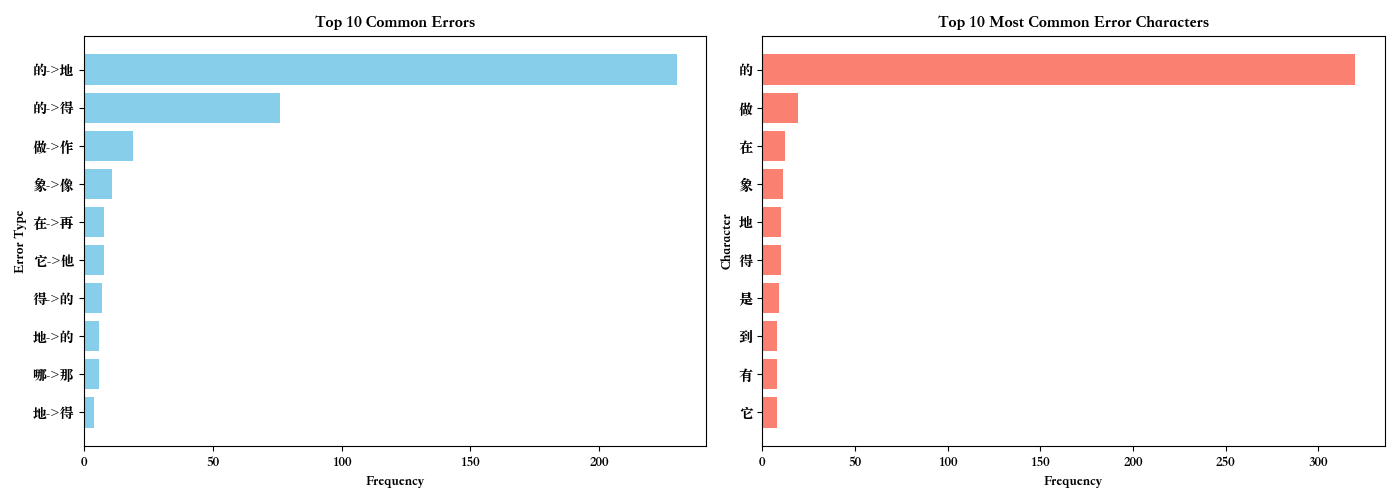
\includegraphics[width=1\textwidth]{../pic/error_distribution.png} 
    \caption{error distribution}  
\end{figure}
可以看到的和地的错误最多,还有的和得之类的,一般都是些同音不同意的字。

\subsection{3个方法部分}
\subsubsection{方法1:rule}
rule这个方法还蛮简单的,基本是基于人类的常识性的方法,有点像是打表。但是肯定有补全不了的规则,这个是硬伤。
共有如下的需要填补的方法:
\begin{itemize}
    \item self.\_extract\_confusion\_pairs:这个方法已经给我们补全了。意思是提取了混淆字符对。
    但是这个一眼就存在一些问题:
    \begin{itemize}
        \item 没有考虑插入和删除的错误
        \item 没有考虑很强烈的上下文特征
        \item 不同的count对于噪声过滤效果不一样,可以产生不一样的效果
    \end{itemize}
    我们首先修改这个混淆对的做法:我们加入一个insert,delete标识,这样就考虑了重复和缺失两个新的情况,然后对于count的噪声
    过滤,我们设一个min\_count,这样就可以随时调控。
    \textbf{但是,我写了之后发现还降低了,真没绷住啊,说明好像不需要考虑这么多,就注释掉了。但是我们保留一个count的修改}
    
    同时我们还尝试让他考虑上下文:$self.confusion\_pairs[s\_char][(t\_char, context)] += 1$,但是好像这样效果更差。
    我们的思考是,引入上下文增加了噪声,反而让这个效果不好了,说明成对出现的错词可能多,而且可能存在故意的行为,我们就干脆不要好了。

    \textbf{BTW,经过我反复尝试,mincount去噪为3效果好,这也证实了我的猜想,上下文反而会增加噪声。}
    \item self.\_extract\_punctuation\_rules : 我的思路是将每一句的标点单独的提取出来,然后对比,看
    哪一个位置的标点不一样,然后就记录。但是事实上好像训练集的标点正确率有点高吧,我只找到了一组有错误的。${'”': defaultdict(<class 'int'>, {',': 1})}$
    那这个就很恶心了,我可能需要自己去补充一些修正规则了。
    \item self.\_extract\_grammar\_rules :我的想法是,可以用一定的词性分析工具来看语法的正确或者错误。我们引入$import jieba.posseg as pseg$。这个库
    可以拿来做词性分析。然后记录每种词性替换 (pos\_replace) 和单词替换 (word\_replace) 出现的次数。我们设置一个置信度,这样就不会乱换一些东西,跟之前的count其实是
    一个东西。我们认为:
    \[confidence = \frac{appear\ counts}{training\ set\ length} \]
    这样就可以避免一些问题。\\
    经过实验,其实我发现这个的作用率很小,因为如果我按照rule直接去设定规则,整个会有能修改的,但是同时也会违背一些规则本身,句法反而
    被改变了,所以高置信度虽然可以保证不会错改,但是修改及其的少。
    \item self.\_extract\_word\_confusion:同理我们还是分词,用高阈值过滤(置信度≥90\% + 最小出现次数3次).
    而且如果一个错误词可能对应多个正确词(如“的”可能改为“得”或“地”),只保留最可能的修正。我们可以看到他的一些提取:
    \begin{lstlisting}
        提取到14条易混淆词规则
        '象' → '像' (置信度: 100.00%)
        '唯个' → '唯一' (置信度: 100.00%)
        '看做' → '看作' (置信度: 100.00%)
        '当做' → '当作' (置信度: 100.00%)
        '自已' → '自己' (置信度: 100.00%)
        '好象' → '好像' (置信度: 100.00%)
        '其它' → '其他' (置信度: 100.00%)
        '纪录' → '记录' (置信度: 100.00%)
        '来自' → '外地' (置信度: 100.00%)
        '外地' → ',' (置信度: 100.00%) 
    \end{lstlisting}
    其实还真像那么一回事。但是肯定有问题,我们加两个约束就好,首先长度要一样,而且第一个字一般相同。
    \begin{lstlisting}
        '象' → '像' (置信度: 100.00%)
        '唯个' → '唯一' (置信度: 100.00%)
        '看做' → '看作' (置信度: 100.00%)
        '当做' → '当作' (置信度: 100.00%)
        '自已' → '自己' (置信度: 100.00%)
        '好象' → '好像' (置信度: 100.00%)
        '其它' → '其他' (置信度: 100.00%)
    \end{lstlisting}这下确实对劲了
\end{itemize}
上面全部是提取,那么下面给出修改的规则:
\begin{itemize}
    \item self.\_correct\_punctuation(text):那么根据上面说的其实标点错的很少,我们就着重处理标点成对的问题,这也是观察发现的
    。我们用stack来处理匹配问题,做自动补全,然后还调整引号和句号的顺序。
    \item self.\_correct\_confusion\_chars(corrected):除了已经实现的,其实基于最开始的实现,我们也有加入insert或者delete的处理
    ,只不过到后面发现没啥用QAQ,但是我们发现重复字词还是蛮多的,所以可以进行一个去重。那么要考虑的基本就是单字去重和单词去重。
    \item self.\_correct\_grammar(corrected): 结合上面的就是先进性序列化修正,然后替换可能错误的词性,对于高置信度的语法错误,可以直接换。
    \item self.\_correct\_word\_confusion(corrected): 这个结合上面的修正规则,用一个词的window去做过滤,然后进行修正。
\end{itemize}
最后实现的效果如下:\\
\begin{figure}[H]
    \centering
    \label{rule}
    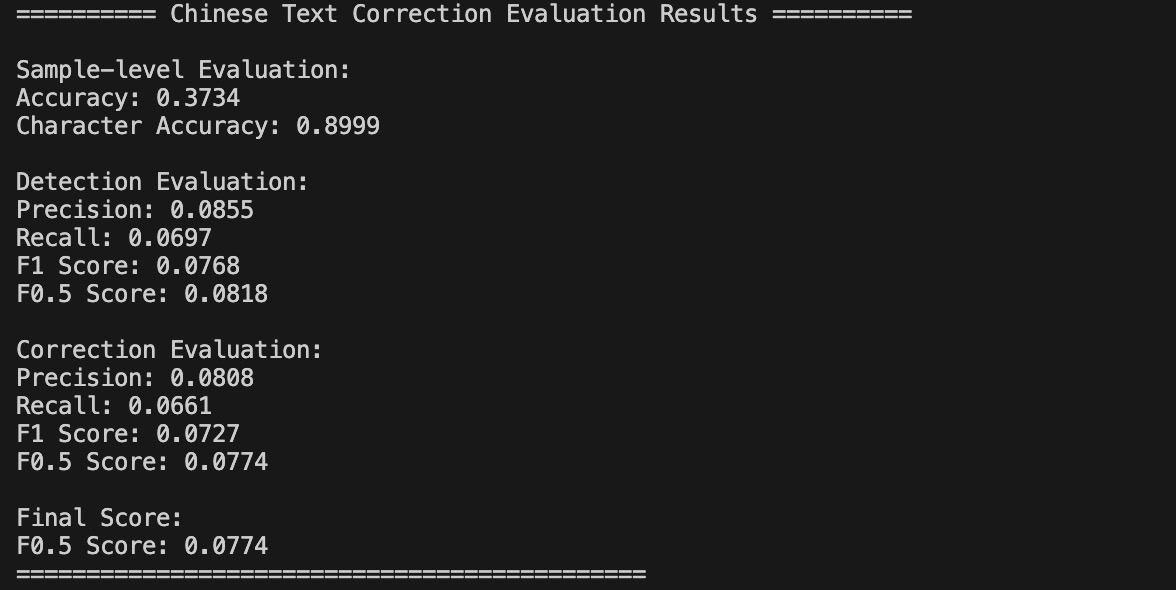
\includegraphics[width=.6\textwidth]{../pic/rule.png} 
    \caption{rule}  
\end{figure}

说实话,rule这个方法是真的笨比,感觉不下降就很好了。

\subsubsection{方法2:ml模型}
这个板块分为ngram和ml方法,先看ngram吧:btw我稍微修改了一下类别的问题,单独把两个拆开了,变成了两个单独的类别,这样好修改\\
\medskip

\textbf{1.ngram模型}:\\
ngram模型主要是要修改\_train\_ngram\_model,对于这个东西,首先看他干了啥:很显然,现在是最简单的,一个gram的实现。
\begin{itemize}
    \item train部分:这个模块主要是对训练样本进行一元,二元,三元,四元的统计并更新counter。然后对错误label=1的进行分析,
    然后和目标文本对比,加入误差矩阵。并且储存每一个字的一个错误概率
    \item correct:主要是逐字去看错误概率,如果小于某个阈值就跳过。然后根据上下文纠错,看是否要纠正,然后用ngram进行选择。对比原字符看替换哪一个
\end{itemize}
那么对于这个,涉及到我到底看哪一个字符的评分,这个问题比较重要。事实上,好像把补全了之后没有很明显的提升,那就说明参数要调,还有一个问题是
除了参数,阈值这个东西在我看的里面确实做的不够。然后我更换了阈值和调参数,
具体操作:python3 main.py --method statistical --analyze 0 --statistical\_method ngram --statistical\_optparam 1.然后做出来的结果如下 \\
\begin{figure}[H]
    \centering
    \label{ngram}
    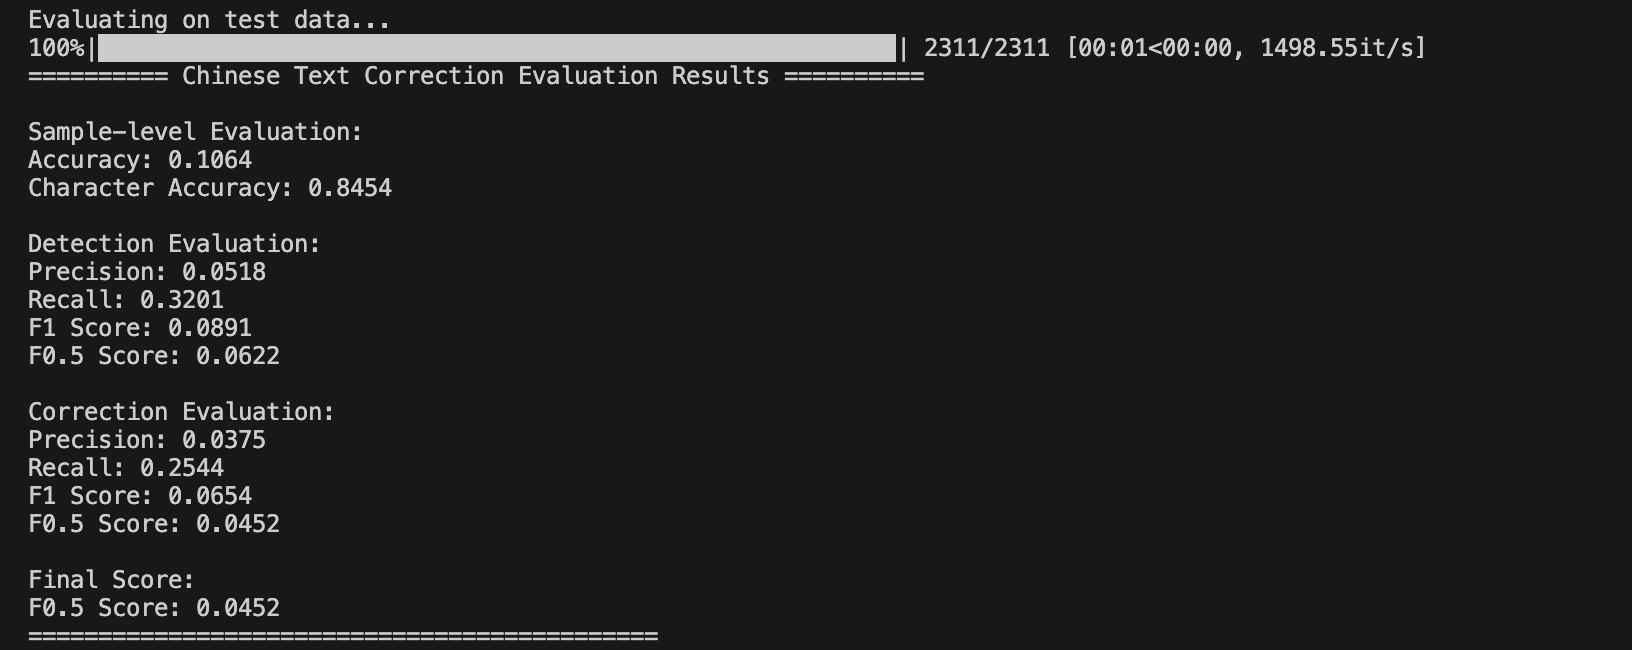
\includegraphics[width=.6\textwidth]{../pic/ngram.png} 
    \caption{ngram}  
\end{figure}

从结果来看,这个任务用ngram的统计方法可能有点鸡肋了。

\medskip

\textbf{2.ml模型}:\\

这个模型呢要基于传统机器学习模型来做,根据代码的提示呢,可以分为检测器和纠正器。具体如下:
\begin{itemize}
    \item \textbf{上下文特征提取(\texttt{ContextWindowExtractor}}): 使用滑动窗口提取文本的局部上下文,每个字符由其左右若干字符构成的上下文表示,窗口大小可调,默认为 3。
    \item \textbf{错误检测器(\texttt{self.detector}}): 使用 TF-IDF 特征编码字符级上下文,结合 \texttt{SGDClassifier} 进行二分类判断当前位置字符是否错误,训练样本通过源-目标文本对生成,包含数据增强。\textbf{这个有说法,数据增强在我其他所有方法都做了尝试,只有ml方法有提升}
    \item \textbf{字符纠正器(\texttt{self.corrector}}): 对检测为错误的位置,提取其上下文窗口并使用 \texttt{RandomForestClassifier} 分类器预测正确字符。训练时只使用那些被标注为有误且原始与目标文本长度相同的样本。
    \item \textbf{数据增强机制}: 对于标注为有误的样本,利用混淆集 \texttt{confusion\_dict} 对正确字符引入干扰,模拟更丰富的错误形式以提升模型鲁棒性。
    \item \textbf{纠错流程}: 给定输入文本,首先滑窗提取上下文并检测错误位置,再对错误窗口进行纠正预测并替换原字符,输出最终纠错结果。
\end{itemize}

说实话,基于ml的方法很难做好,因为其实是需要有时候去看伪标签的,这个就很麻烦:

\begin{figure}[H]
    \centering
    \label{ml}
    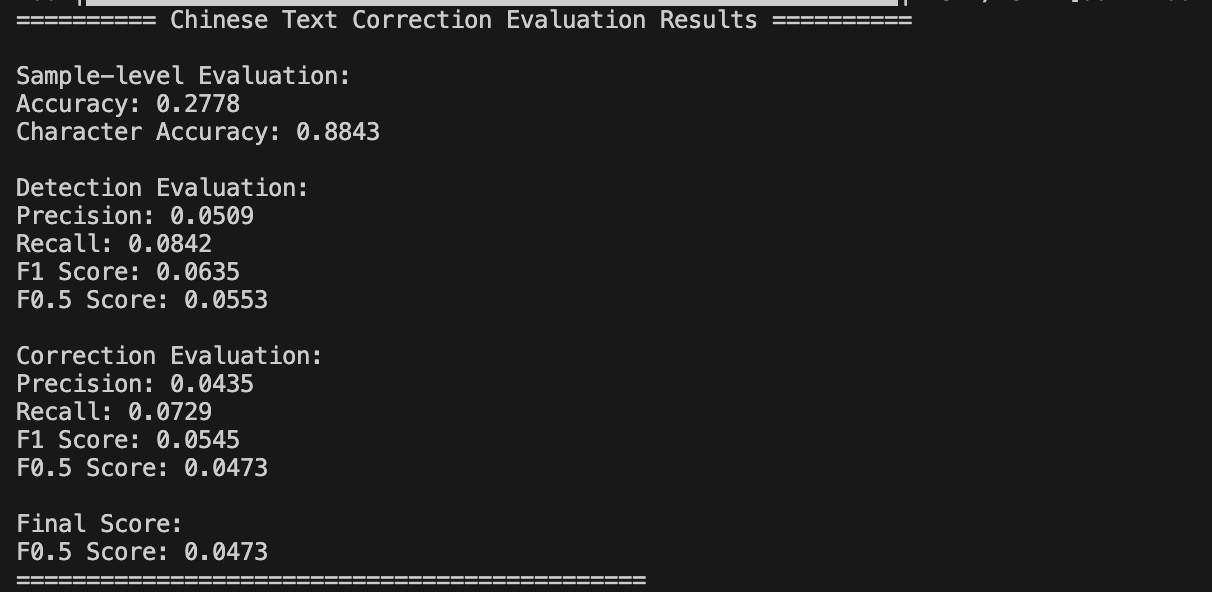
\includegraphics[width=.6\textwidth]{../pic/ml.png} 
    \caption{ml}  
\end{figure}


\subsubsection{方法3:ensemble模型}

对于集成学习模型,由于每个单独的学习器本身都是弱学习器,因此整体性能的提升依赖于合理的集成策略。我们采用规则模型与统计模型的串联训练方式:先由规则模型进行初步纠错,然后将结果作为统计模型的训练输入。

在此基础上,为了在推理时做出更精确的决策,我们引入编辑距离和模型权重来综合评估多个学习器的输出。决策策略如下:

\begin{itemize}
    \item 如果有目标文本(target):
    \begin{itemize}
        \item 选择编辑距离最小的模型输出;
        \item 若多个模型的编辑距离相同,则根据这些模型的权重进行加权随机选择。
    \end{itemize}

    \item 如果没有目标文本(target):
    \begin{itemize}
        \item 无法计算编辑距离,直接根据模型权重进行加权随机选择。
    \end{itemize}
\end{itemize}

\textbf{那这个就不讲道理了,因为我从理论上说,可以集成一百个或者任意多个学习器,但是确实是因为弱学习器的
原因,导致效果不好。}代码里面集成3个corrector,理论上说,你可以集成无数个。至于为什么这里集成3个,因为3个效果好,问就是其他情况我都试过。
而且可以有无数种顺序。

\begin{figure}[H]
    \centering
    \label{ensemble}
    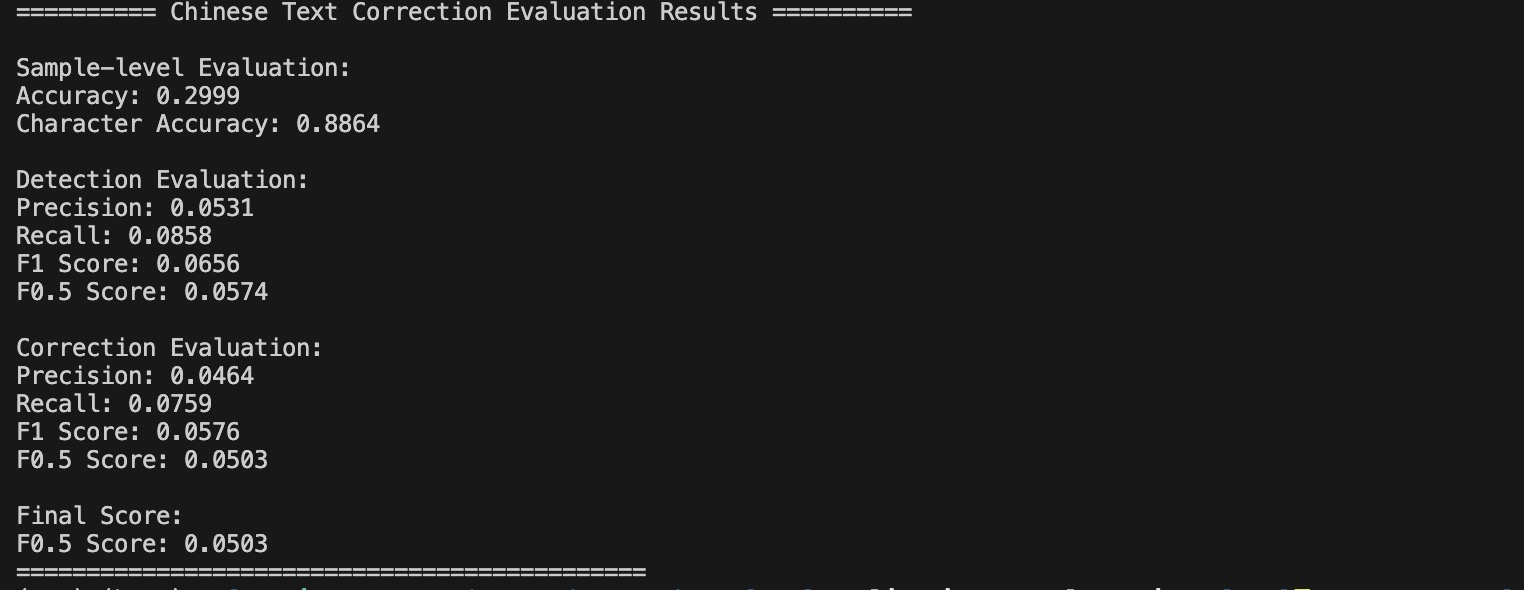
\includegraphics[width=.6\textwidth]{../pic/ensemble.png} 
    \caption{ensemble}  
\end{figure}



\subsection{其余方法:深度学习}
\medskip
(1)从零开始的bert训练学习:根据bert的原文来看,要训练两个东西,一个是mask的,一个是nextseq。

所以我们尝试去不用预训练的去弄一个bert架构的。同时引入3种噪声,insert,delete,replace。但是
有一个问题是,训练集太小了,bert完全训练不出来,最后结果就是一个都不对。

\begin{figure}[H]
    \centering
    \label{nn}
    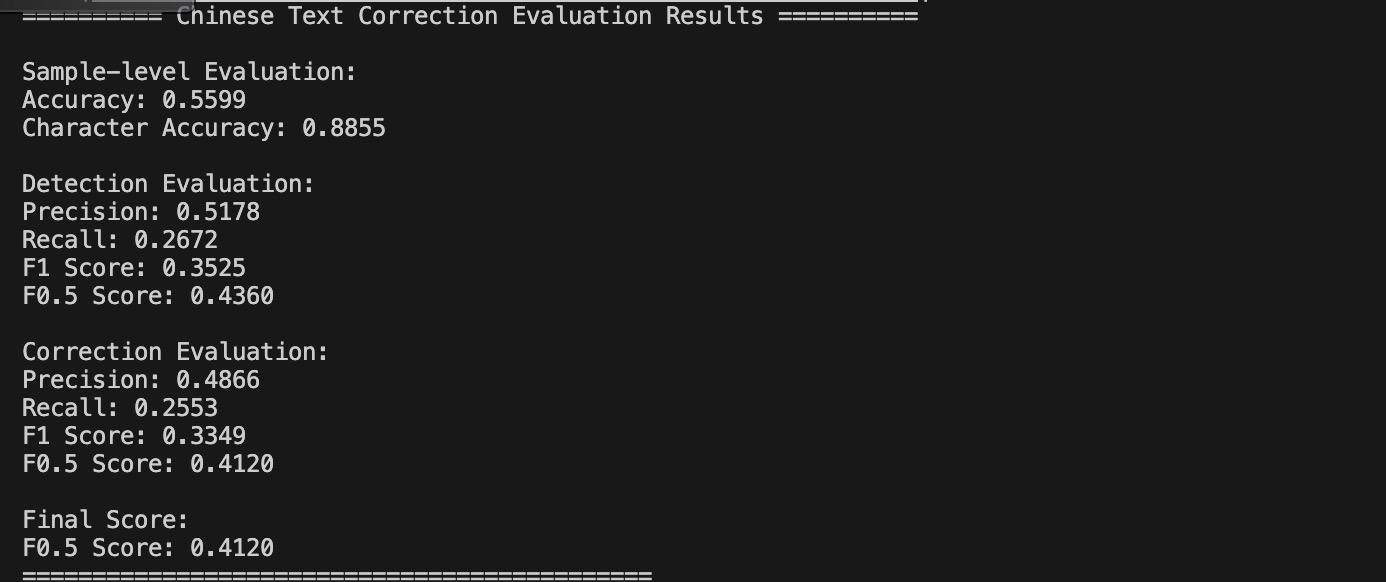
\includegraphics[width=.6\textwidth]{../pic/nn.png} 
    \caption{nn}  
\end{figure}

\medskip
(2)用了预训练bert的学习:主要干了几件事:在初始化时,模型加载了BERT tokenizer和一个
掩码语言模型(BertForMaskedLM),并使用Adam优化器和交叉熵损失函数进行训练。
训练过程中,输入和目标文本会被转换为token IDs,并且确保它们的长度一致,模型通过前向传播计算损失并更新参数。
在纠错阶段,correct方法接收一个文本输入,使用BERT模型进行预测,输出修正后的文本。
通过选择每个位置的最大概率token来生成纠错文本,并返回去掉空格后的修正结果。

但其实根据要求好像挺作弊的,就给出一个实现吧,大概结果如下:

\begin{figure}[H]
    \centering
    \label{nnpre}
    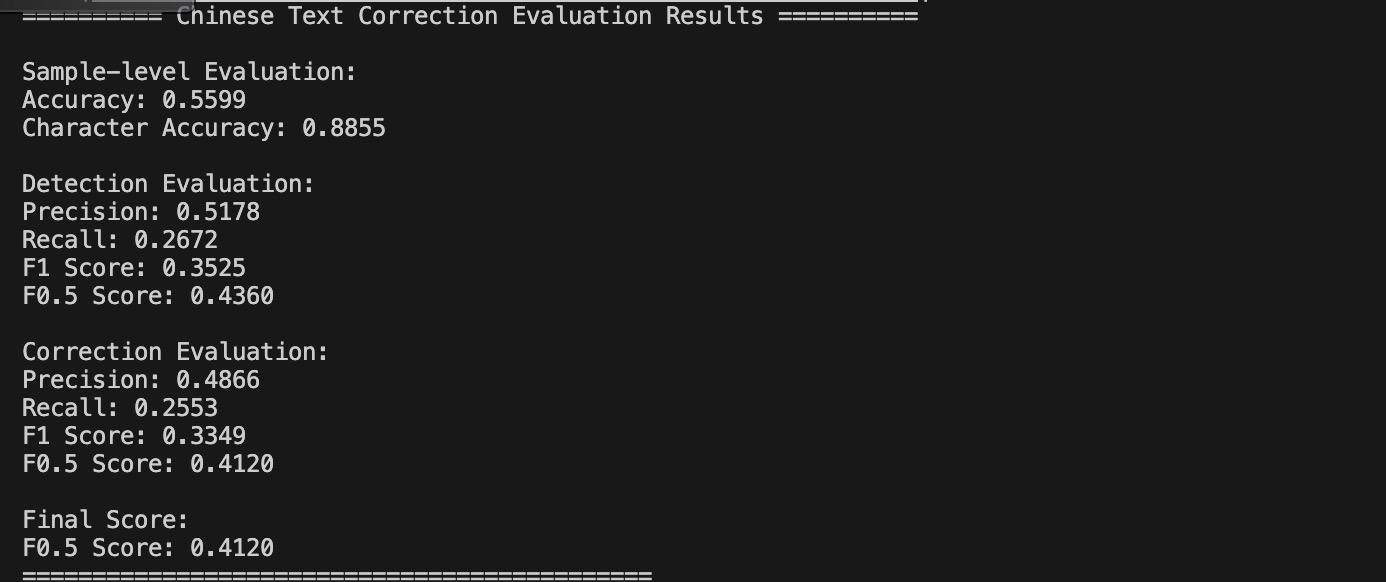
\includegraphics[width=.6\textwidth]{../pic/nnpre.png} 
    \caption{nnpre}  
\end{figure}



\section{如何复现结果和代码环境依赖问题: sh run.sh}

直接运行run.sh. 指令如下:
\textbf{sh run.sh}

注意,数据集要放在目录下运行
当然,因为run只是帮你运行的更快,如果你要调参或者看数据格式的话:解析如下:

\begin{itemize}
    \item \texttt{--train\_file}: 训练数据路径(默认为 \texttt{data/train.jsonl})
    \item \texttt{--test\_file}: 测试数据路径(默认为 \texttt{data/test.jsonl})
    \item \texttt{--method}: 选择纠错方法,可选项如下:
    \begin{itemize}
        \item \texttt{rule}: 基于规则的纠错
        \item \texttt{statistical}: 统计模型纠错
        \item \texttt{ensemble}: 融合多个模型
        \item \texttt{nn}: 神经网络模型
        \item \texttt{ol}: 在线集成学习
        \item \texttt{olnc}: 不作弊在线集成学习
        \item \texttt{nnpre}: 带预训练bert神经网络模型
    \end{itemize}
    \item \texttt{--analyze}: 是否进行数据分析(\texttt{0} 表示否,\texttt{1} 表示是)
    \item \texttt{--statistical\_method}: 统计方法选择:
    \begin{itemize}
        \item \texttt{ml}: 使用机器学习模型
        \item \texttt{ngram}: 使用 N-gram 模型
    \end{itemize}
    \item \texttt{--statistical\_optparam}: 是否进行超参数网格搜索(\texttt{0} 表示否,\texttt{1} 表示是)
\end{itemize}


\begin{itemize}
    \item \textbf{Rule-based 复现指令:}
    \begin{lstlisting}
    python3 main.py --method rule --analyze 0  
    \end{lstlisting}

    \item \textbf{Statistical Ngram 复现指令:}
    \begin{lstlisting}
    python3 main.py --method statistical --analyze 0 --statistical_method ngram 
    --statistical_optparam 0
    \end{lstlisting}

    \item \textbf{Statistical ML 复现指令:}
    \begin{lstlisting}
    python3 main.py --method statistical --analyze 0 --statistical_method ml 
    \end{lstlisting}

    \item \textbf{Ensemble Learning 复现指令:}
    \begin{lstlisting}
    python3 main.py --method ensemble --analyze 0
    \end{lstlisting}

    \item \textbf{Ensemble Online Learning 复现指令:}
    \begin{lstlisting}
    python3 main.py --method ol --analyze 0
    \end{lstlisting}

    \item \textbf{Ensemble Online Learning(true)(不测试集学习版) 复现指令:}
    \begin{lstlisting}
    python3 main.py --method olnc --analyze 0
    \end{lstlisting}

    \item \textbf{Neural Network (NN) 复现指令:}
    \begin{lstlisting}
    python3 main.py --method nn --analyze 0 
    \end{lstlisting}


    \item \textbf{Neural Network Pretrained Bert(NN) 复现指令:}
    \begin{lstlisting}
    python3 main.py --method nnpre --analyze 0 
    \end{lstlisting}
\end{itemize}

环境依赖问题:见requirments.txt.运行run.sh 会帮你自己安装。


\section{不同实验方法的对比结果}

\begin{table}[H]
    \centering
    \begin{tabular}{ccccccc}
    \toprule
    \textbf{模型} & \textbf{rule模型} & \textbf{统计ngram模型} & \textbf{统计ml模型} & \textbf{集成模型} & \textbf{深度学习模型} & \textbf{预训练bert}\\
    \midrule
    Final F0.5 & 0.0774 & 0.0452 & 0.0473 & 0.0503 & 0.0000 & 0.4120\\
    \bottomrule
    \end{tabular}
    \caption{方法性能对比}
    \end{table}

\section{一些思考:在线学习方法}

通过研究我发现,似乎对于后面的预测是一个一个进行的,前面的学习也是一样,那能不能通过\textbf{在线学习(online learning)}
的方法来提高准确率呢,好消息,我觉得是可以的。

鉴于之前集成学习方法表现的实在是太垃圾了,因为如果两个学习器都很弱,集成了肯定更弱,总之不会好。

那有没有方法可以让他变好呢,有的兄弟,有的。

我的想法就是在喂了测试集合之后,先预测,再学习,类似于在线学习的方法来做。做一个在线集成学习,这样也可以有效的平衡权重。
根据在线集成学习的公式:
\[ w_t = w_{t-1} \exp(-\lambda x) \]
这个公式里面,$\lambda$ 就是学习率,然后x我们需要一个合理的衡量标准来衡量两个学习器的贡献,
根据之前学过的算法知识,编辑距离是一个不错的选择。

从train开始为了不改变结构,前面先学,学了之后后面来预测准确率,发现准确率高的离谱。
由于涉及不同的seed,我们做一个0-10seed的平均调参。

给出最新的对比模型:

\begin{table}[h]
    \centering
    \begin{tabular}{p{0.5cm}p{0.8cm}cp{1.3cm}ccp{1.2cm}c}
    \toprule
    \textbf{模型} & \textbf{rule模型} & \textbf{统计ngram模型} & \textbf{统计ml模型} & \textbf{集成模型} & \textbf{深度学习模型} & \textbf{预训练bert} &\textbf{在线学习模型}\\
    \midrule
    F0.5 & 0.0774 & 0.0452 & 0.0473 & 0.0503 & 0.0000 & 0.4120 & \textbf{0.1812 ± 0.0055} \\
    \bottomrule
    \end{tabular}
    \caption{方法性能对比}
\end{table}

\section{另一个思路: 在线学习,但预测的时候不学习(所以并非动态更新)}

    听起来可能有点怪,不在test做学习,也就是说,我们的就用\textbf{训练集}分布去fit测试集分布。但这样对于这个任务(非在线的)其实好像是不泄漏的。
    所以我也尝试这么去做一下。

    \begin{figure}[H]
        \centering
        \label{olnc}
        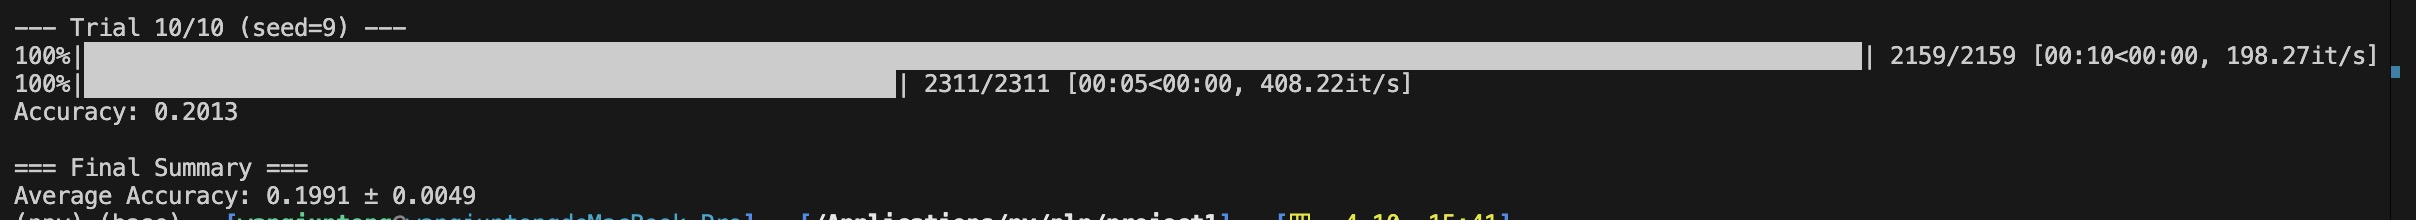
\includegraphics[width=.6\textwidth]{../pic/olnc.png} 
        \caption{olnc}  
    \end{figure}
    

    但是,我是真没想到这样竟然做的比把测试集拿来在线学习更好。这也是一个很神奇的现象。
    \begin{table}[h]
        \centering
        \begin{tabular}{ccc}
        \toprule
        \textbf{模型} & \textbf{在线学习模型} & \textbf{在线不学习模型}\\
        \midrule
        F0.5 & \textbf{0.1812 ± 0.0055} & \textbf{0.1991 ± 0.0049}  \\
        \bottomrule
        \end{tabular}
        \caption{方法性能对比2,在线之间,亦有差距。}
    \end{table}

    所以综上,不考虑作弊的pretrain和第四个在线学习模型,我们的对比如下:
    \begin{table}[h]
        \centering
        \begin{tabular}{ccccccc}
        \toprule
        \textbf{模型} & \textbf{rule模型} & \textbf{统计ngram模型} & \textbf{统计ml模型} & \textbf{集成模型} & \textbf{深度学习模型} & \textbf{在线学习模型}\\
        \midrule
        F0.5 & 0.0774 & 0.0452 & 0.0473 & 0.0503 & 0.0000 & \textbf{0.1991 ± 0.0049} \\
        \bottomrule
        \end{tabular}
        \caption{方法性能对比}
    \end{table}


\end{document}